\chapter{Cristales semiconductores} \label{Ch:09}

\section{Concetración de portadores en equilibrio térmico}

\section{Semiconductores dopados}

\section{Concentración de portadores en Semiconductores dopados}

\section{Conductividad y movilidad}

\section{Semiconductores inhomogeneos: la unión p-n.}
\begin{figure}[h!] \centering
	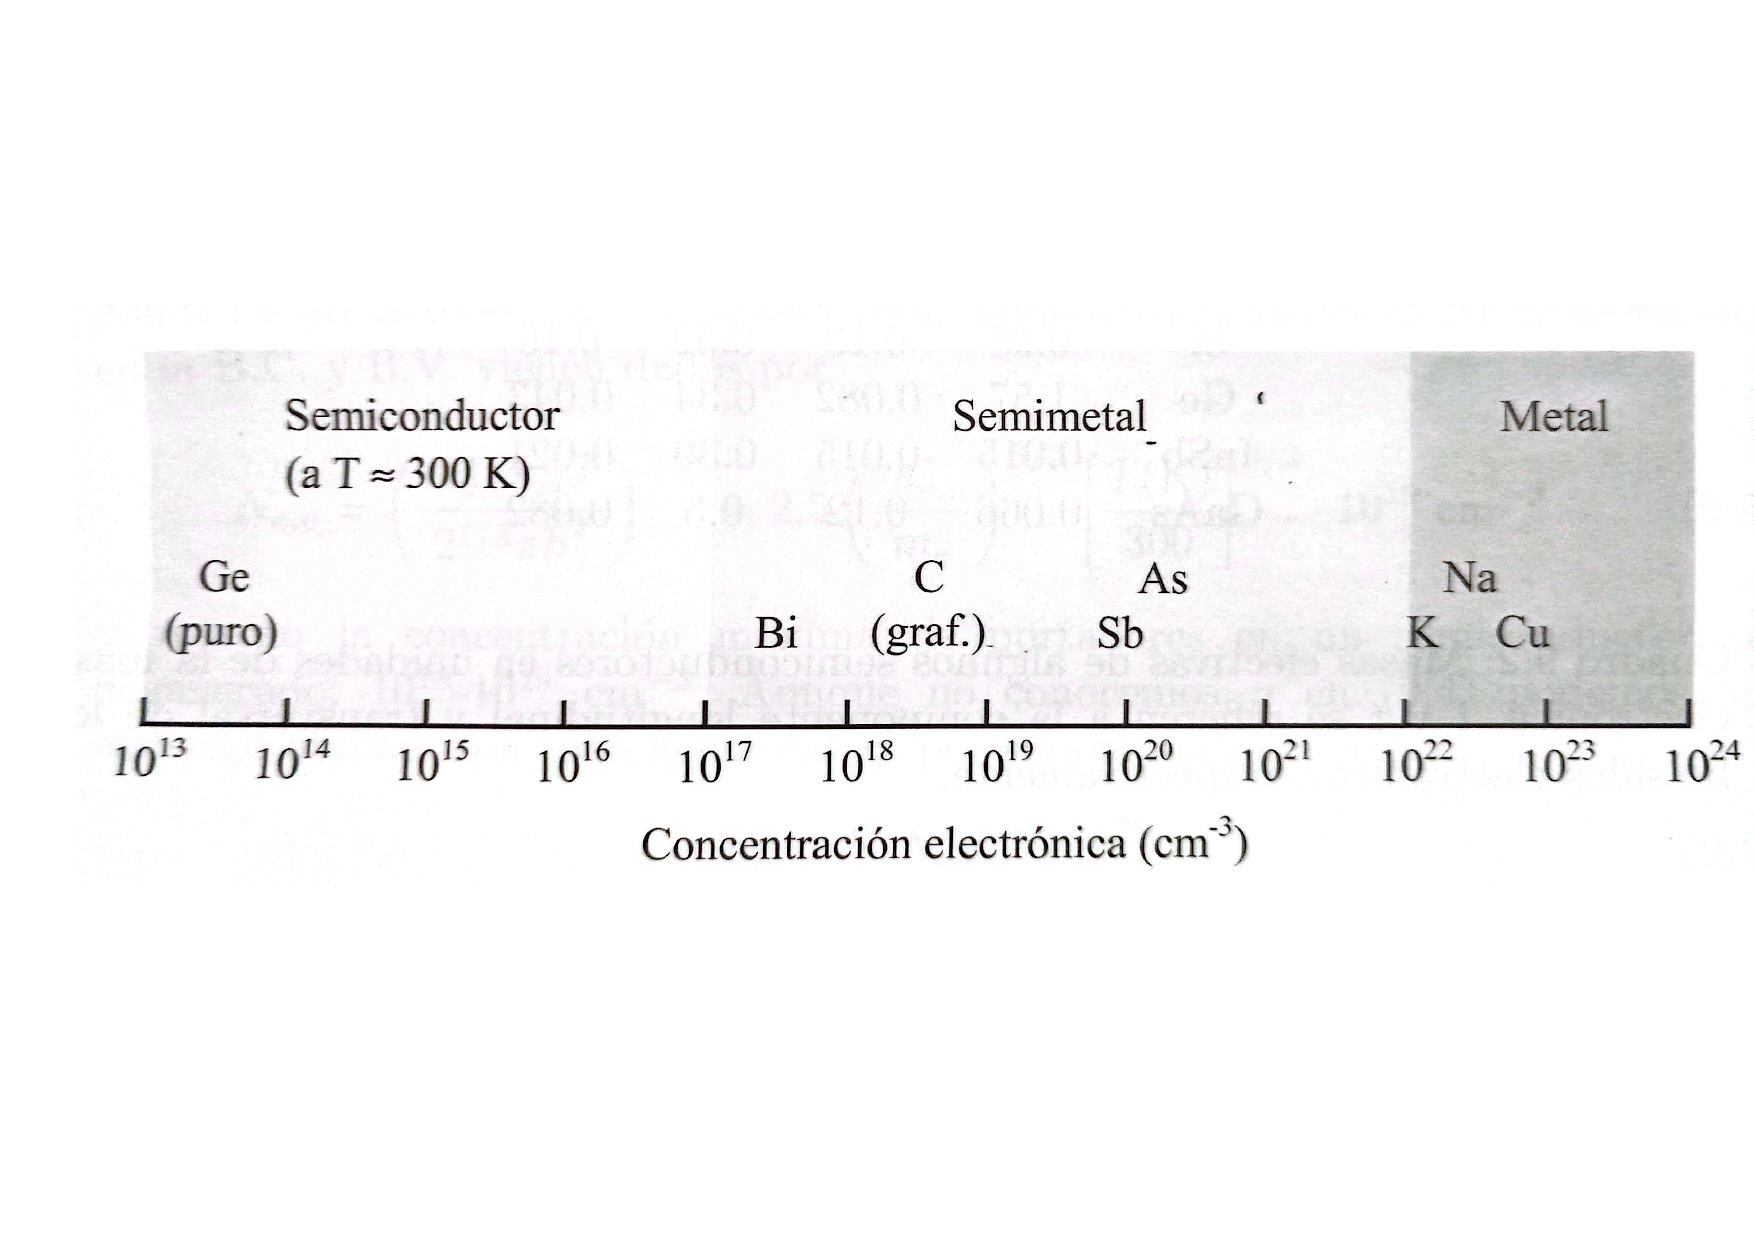
\includegraphics[scale=0.5]{Cuerpo/Ch_09/Fotos libro 1.pdf}
	\caption{}
	\label{Fig:09-01}
\end{figure}
\begin{figure}[h!] \centering
	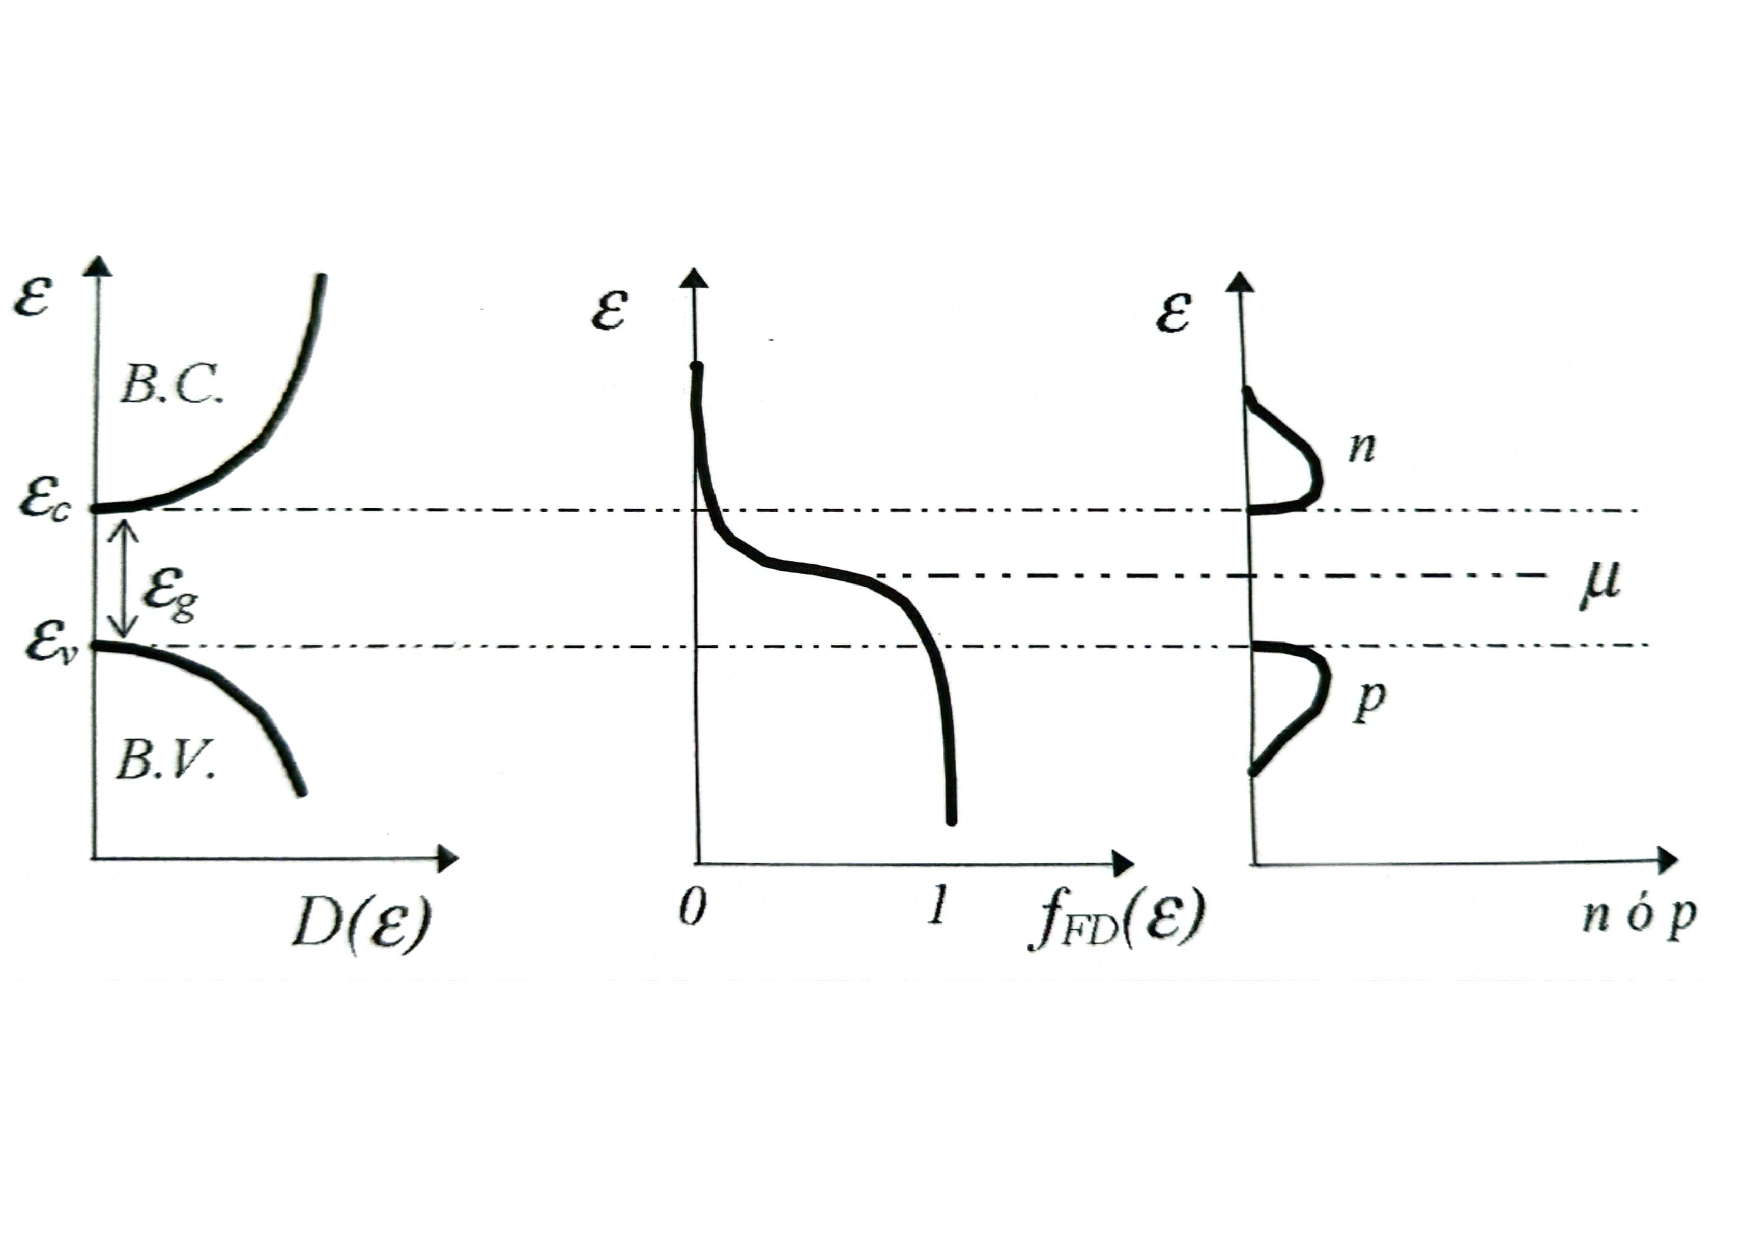
\includegraphics[scale=0.5]{Cuerpo/Ch_09/Fotos libro 2.pdf}
	\caption{}
	\label{Fig:09-02}
\end{figure}
\begin{figure}[h!] \centering
	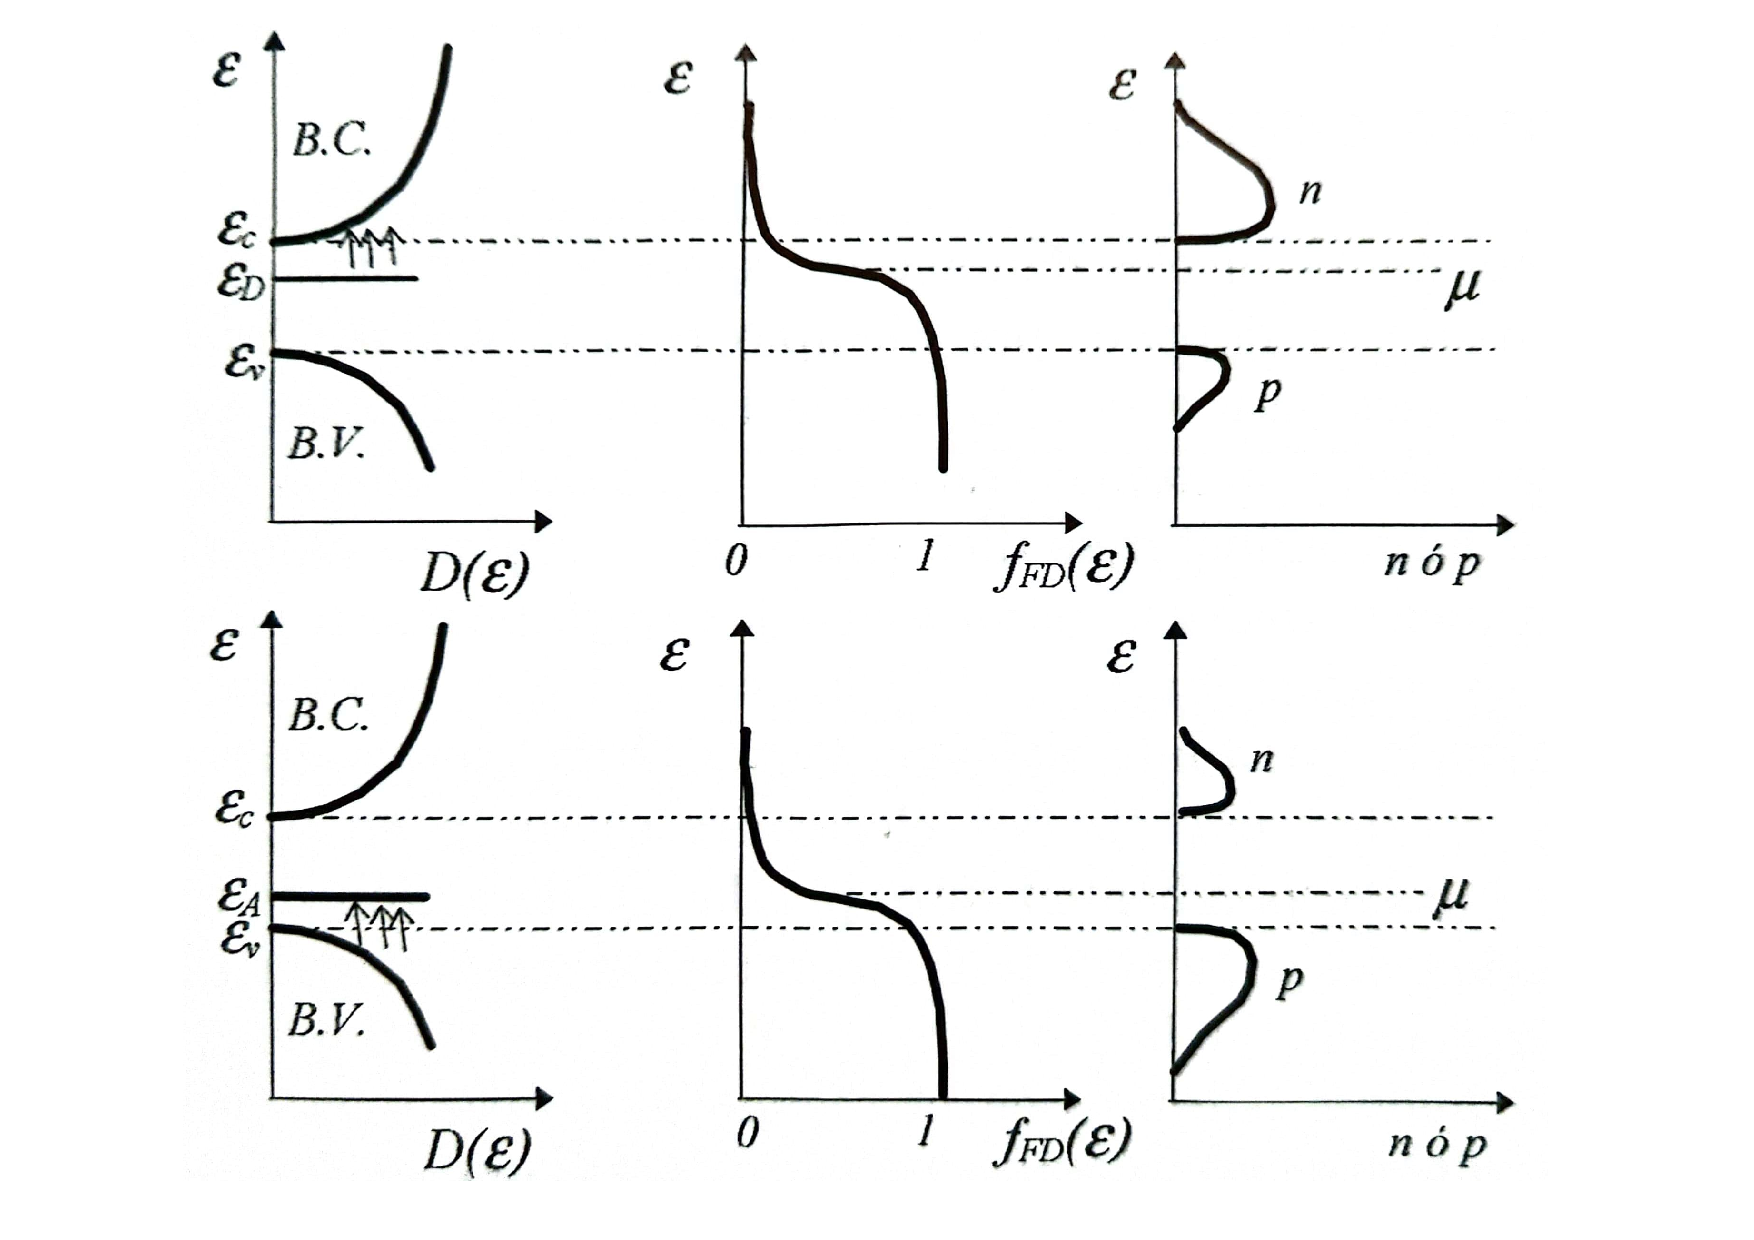
\includegraphics[scale=0.5]{Cuerpo/Ch_09/Fotos libro 3.pdf}
	\caption{}
	\label{Fig:09-03}
\end{figure}
\begin{figure}[h!] \centering
	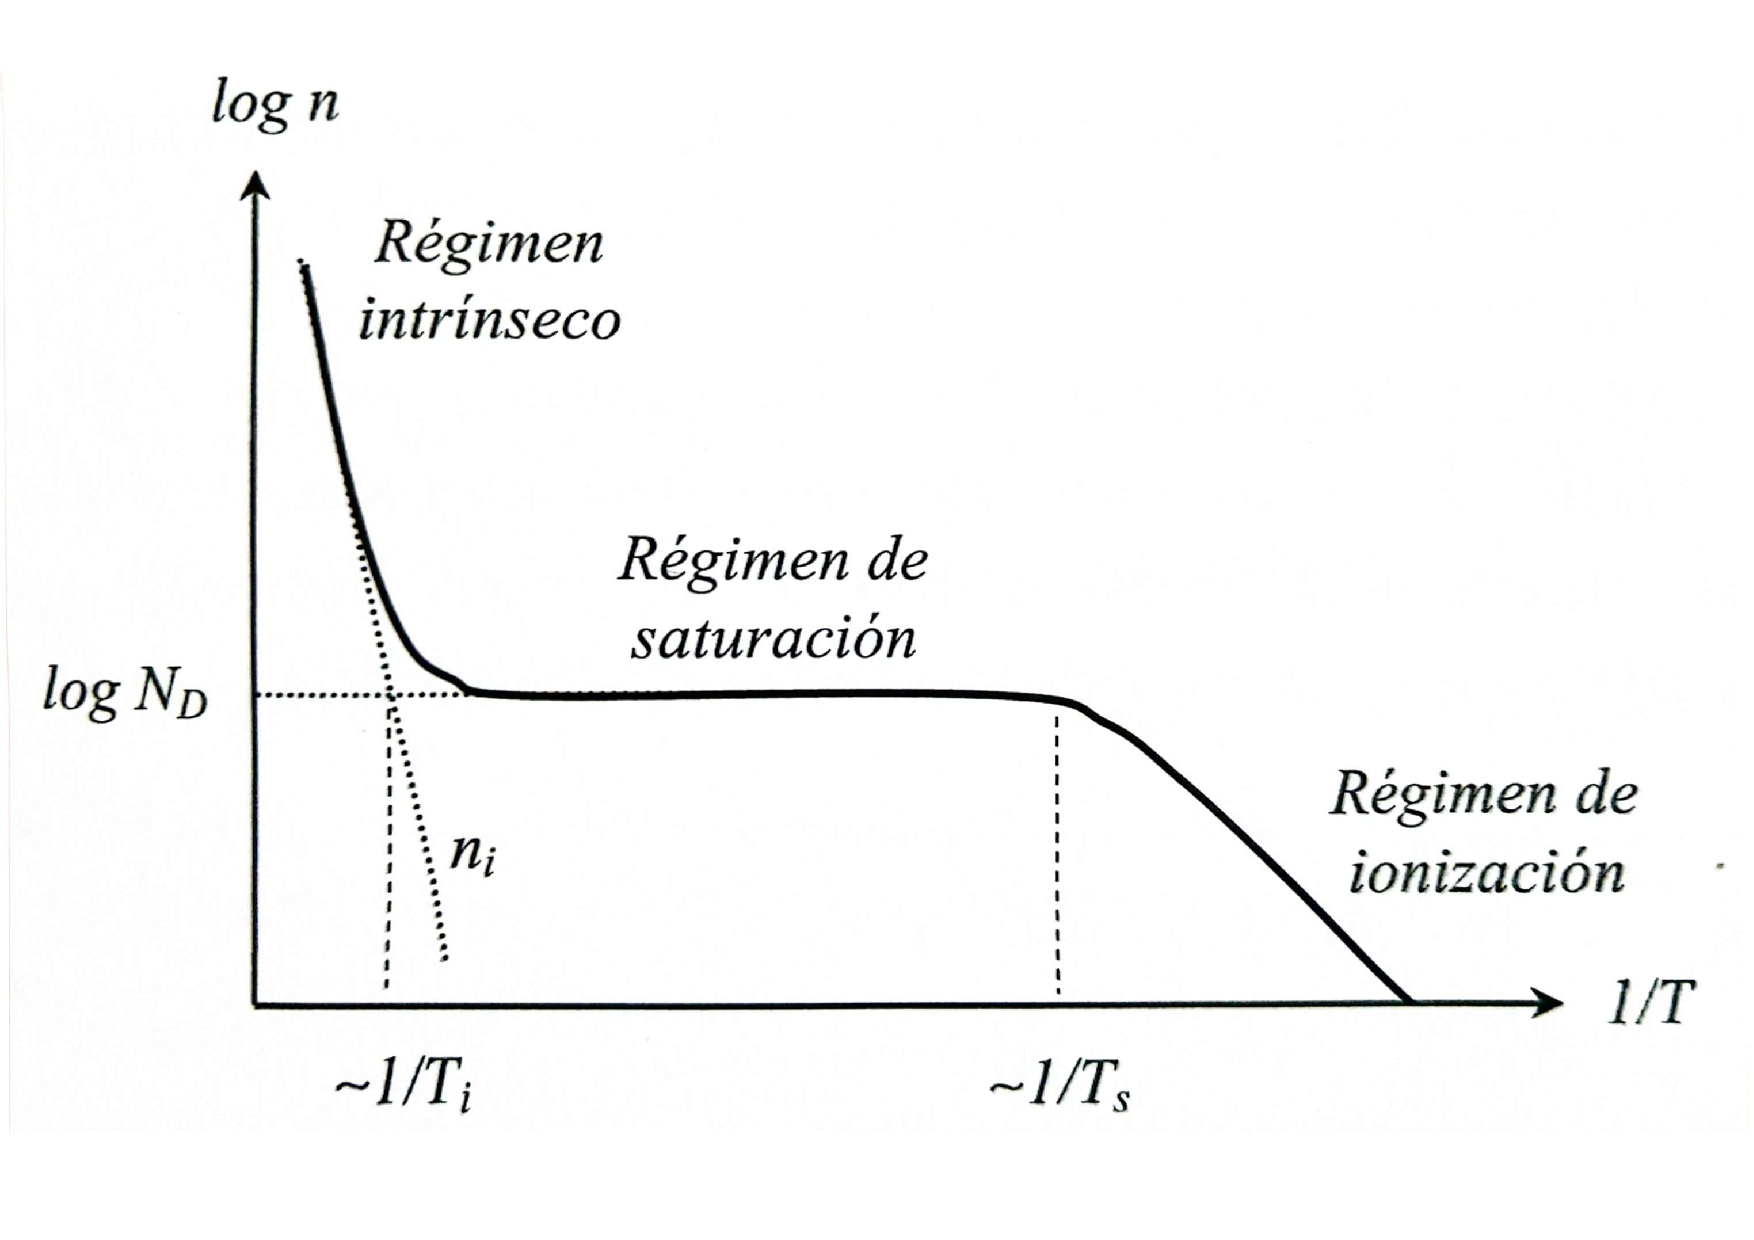
\includegraphics[scale=0.5]{Cuerpo/Ch_09/Fotos libro 4.pdf}
	\caption{}
	\label{Fig:09-04}
\end{figure}
\begin{figure}[h!] \centering
	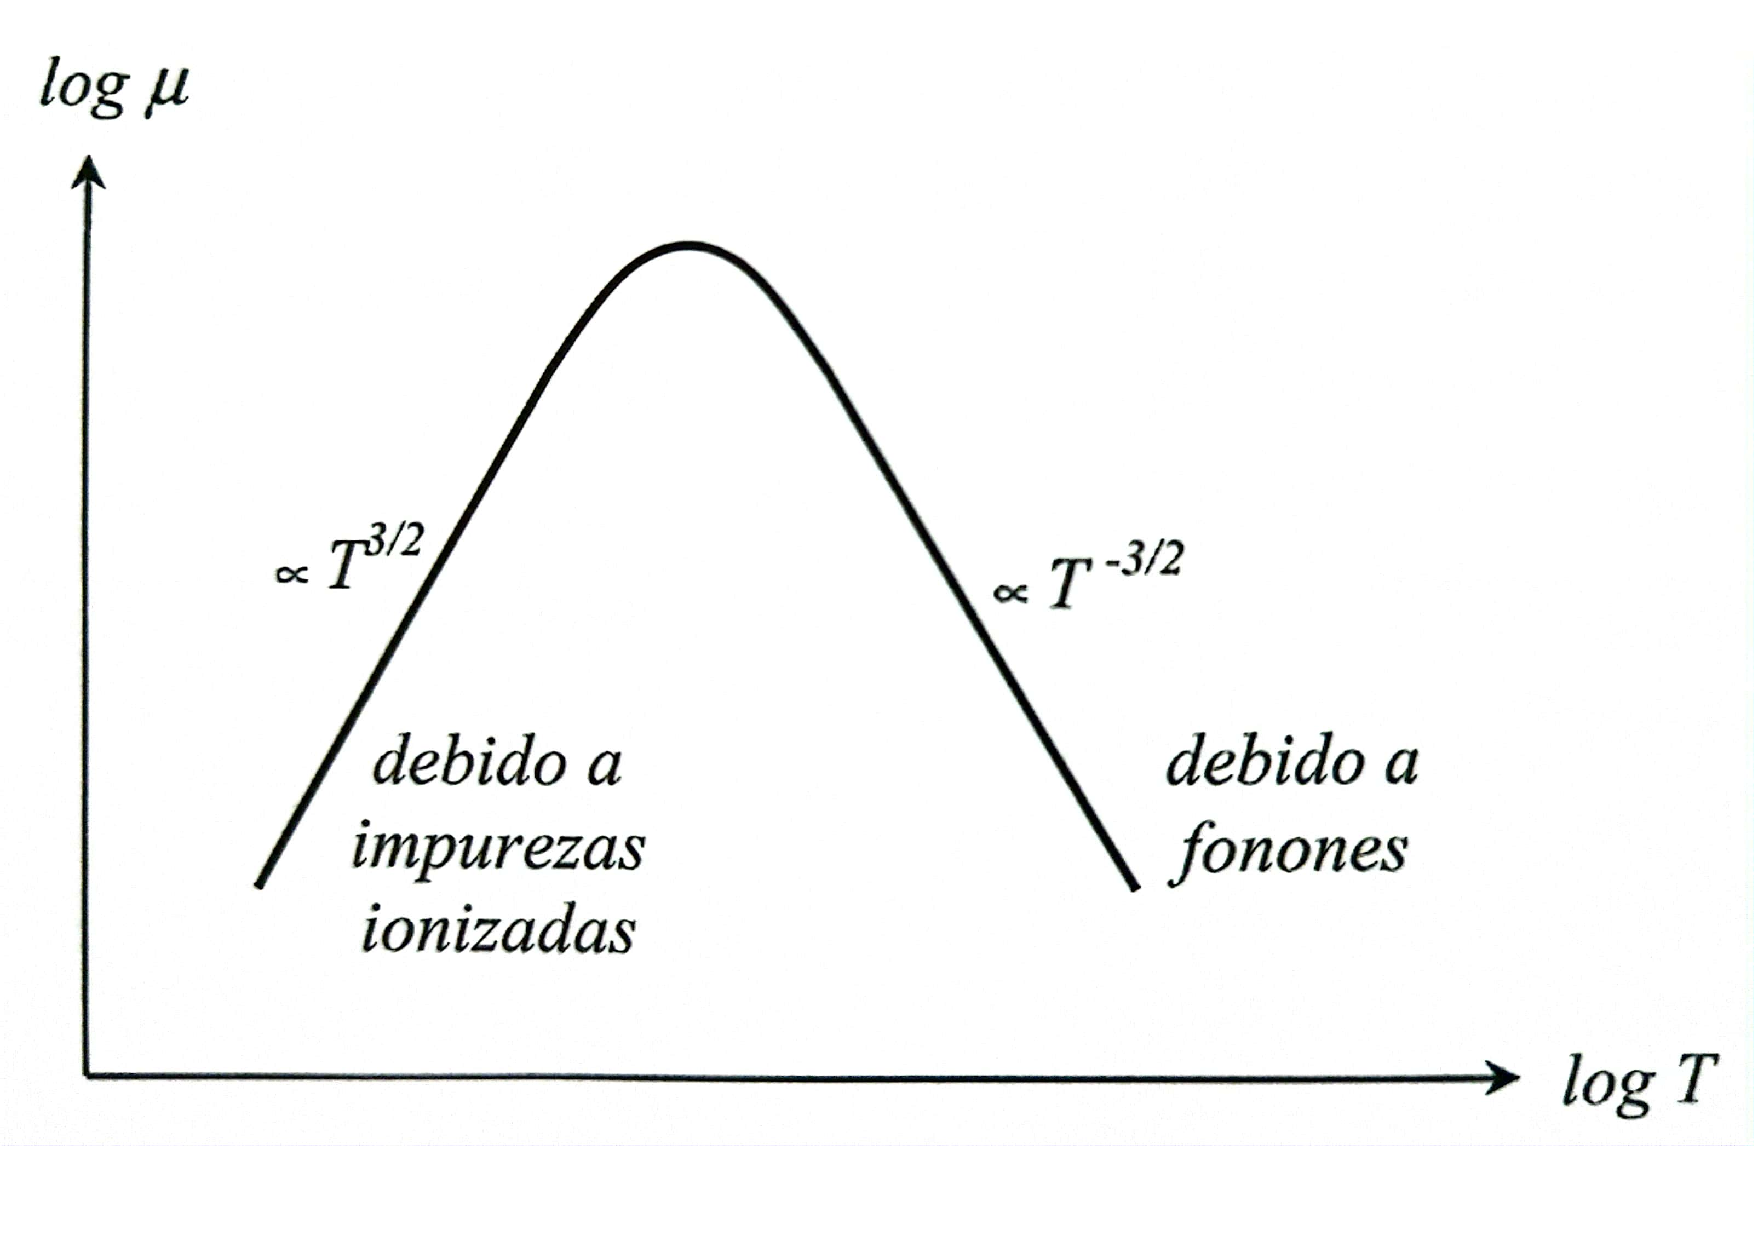
\includegraphics[scale=0.5]{Cuerpo/Ch_09/Fotos libro 5.pdf}
	\caption{}
	\label{Fig:09-05}
\end{figure}
\begin{figure}[h!] \centering
	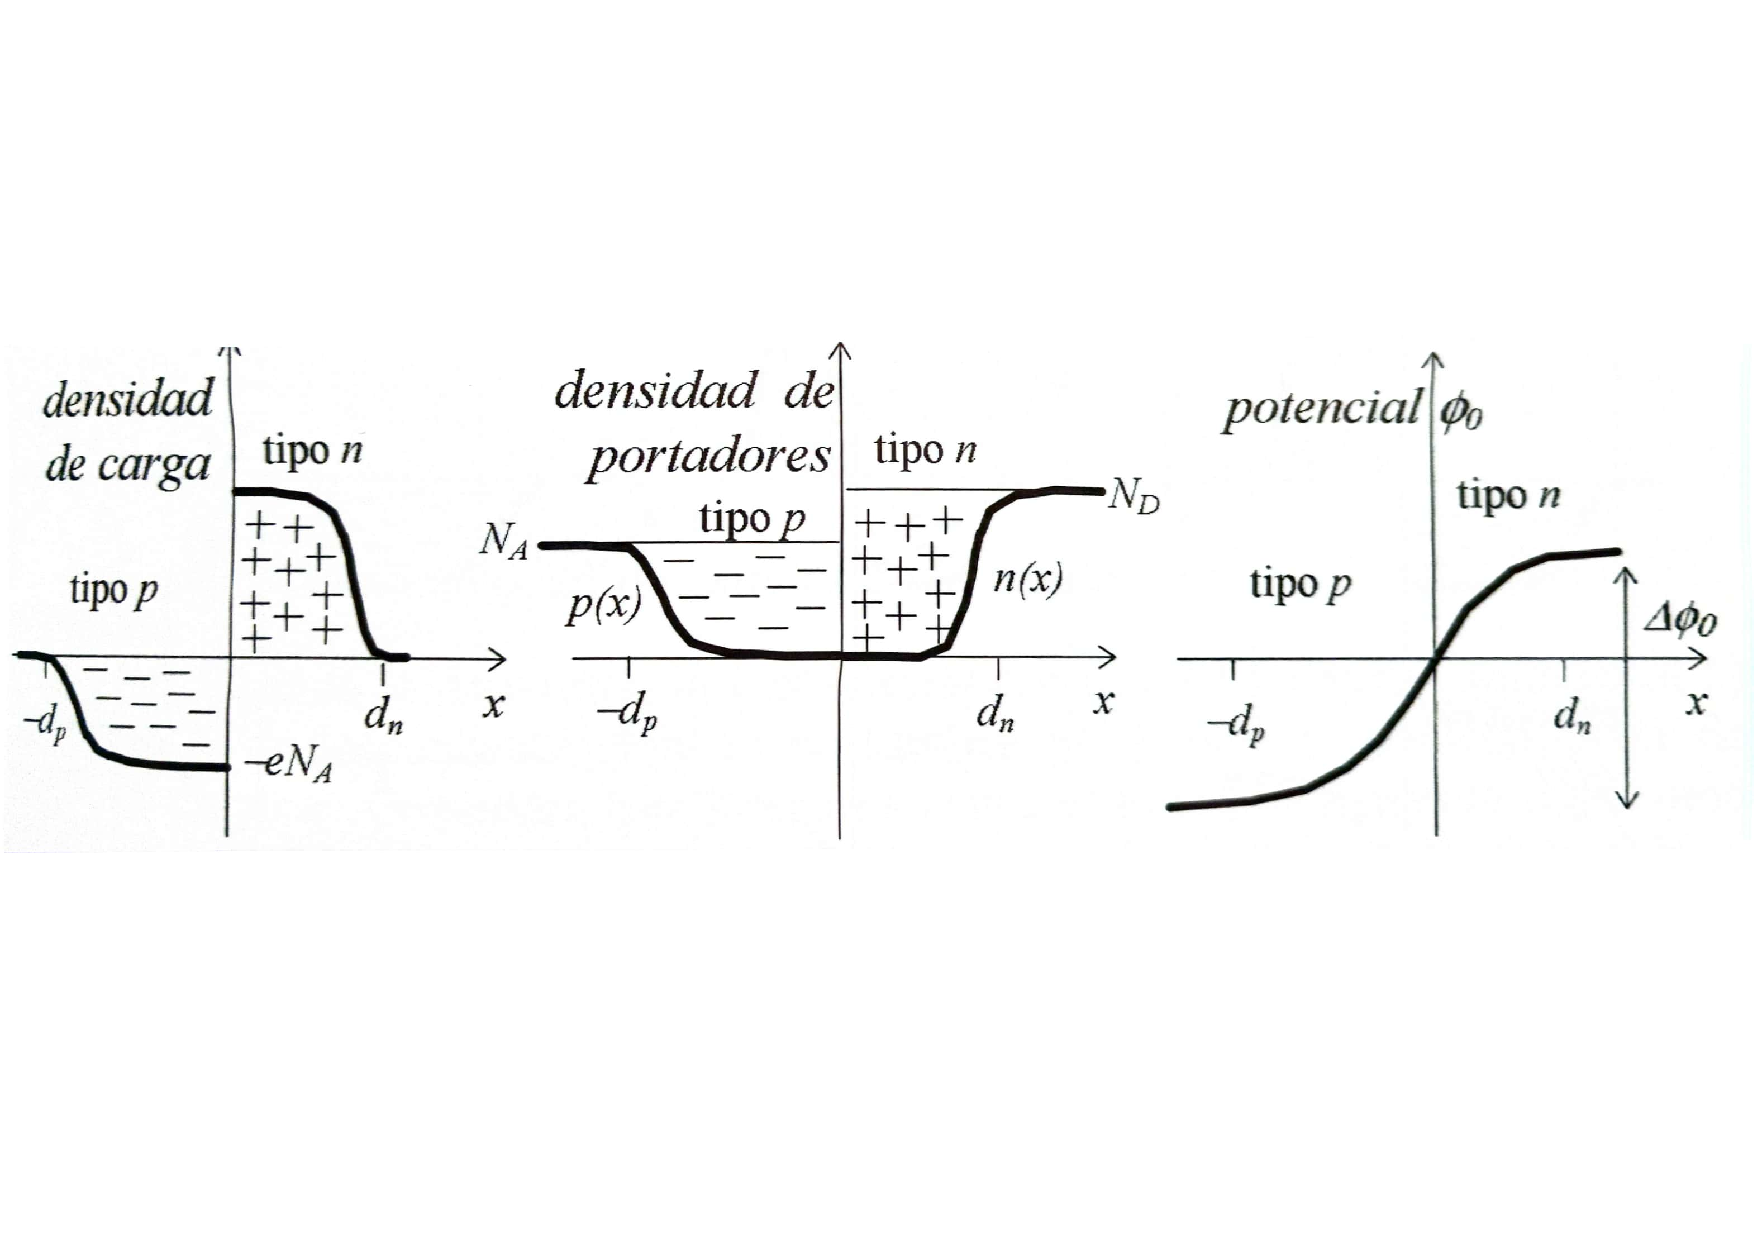
\includegraphics[scale=0.5]{Cuerpo/Ch_09/Fotos libro 6.pdf}
	\caption{}
	\label{Fig:09-06}
\end{figure}
\begin{figure}[h!] \centering
	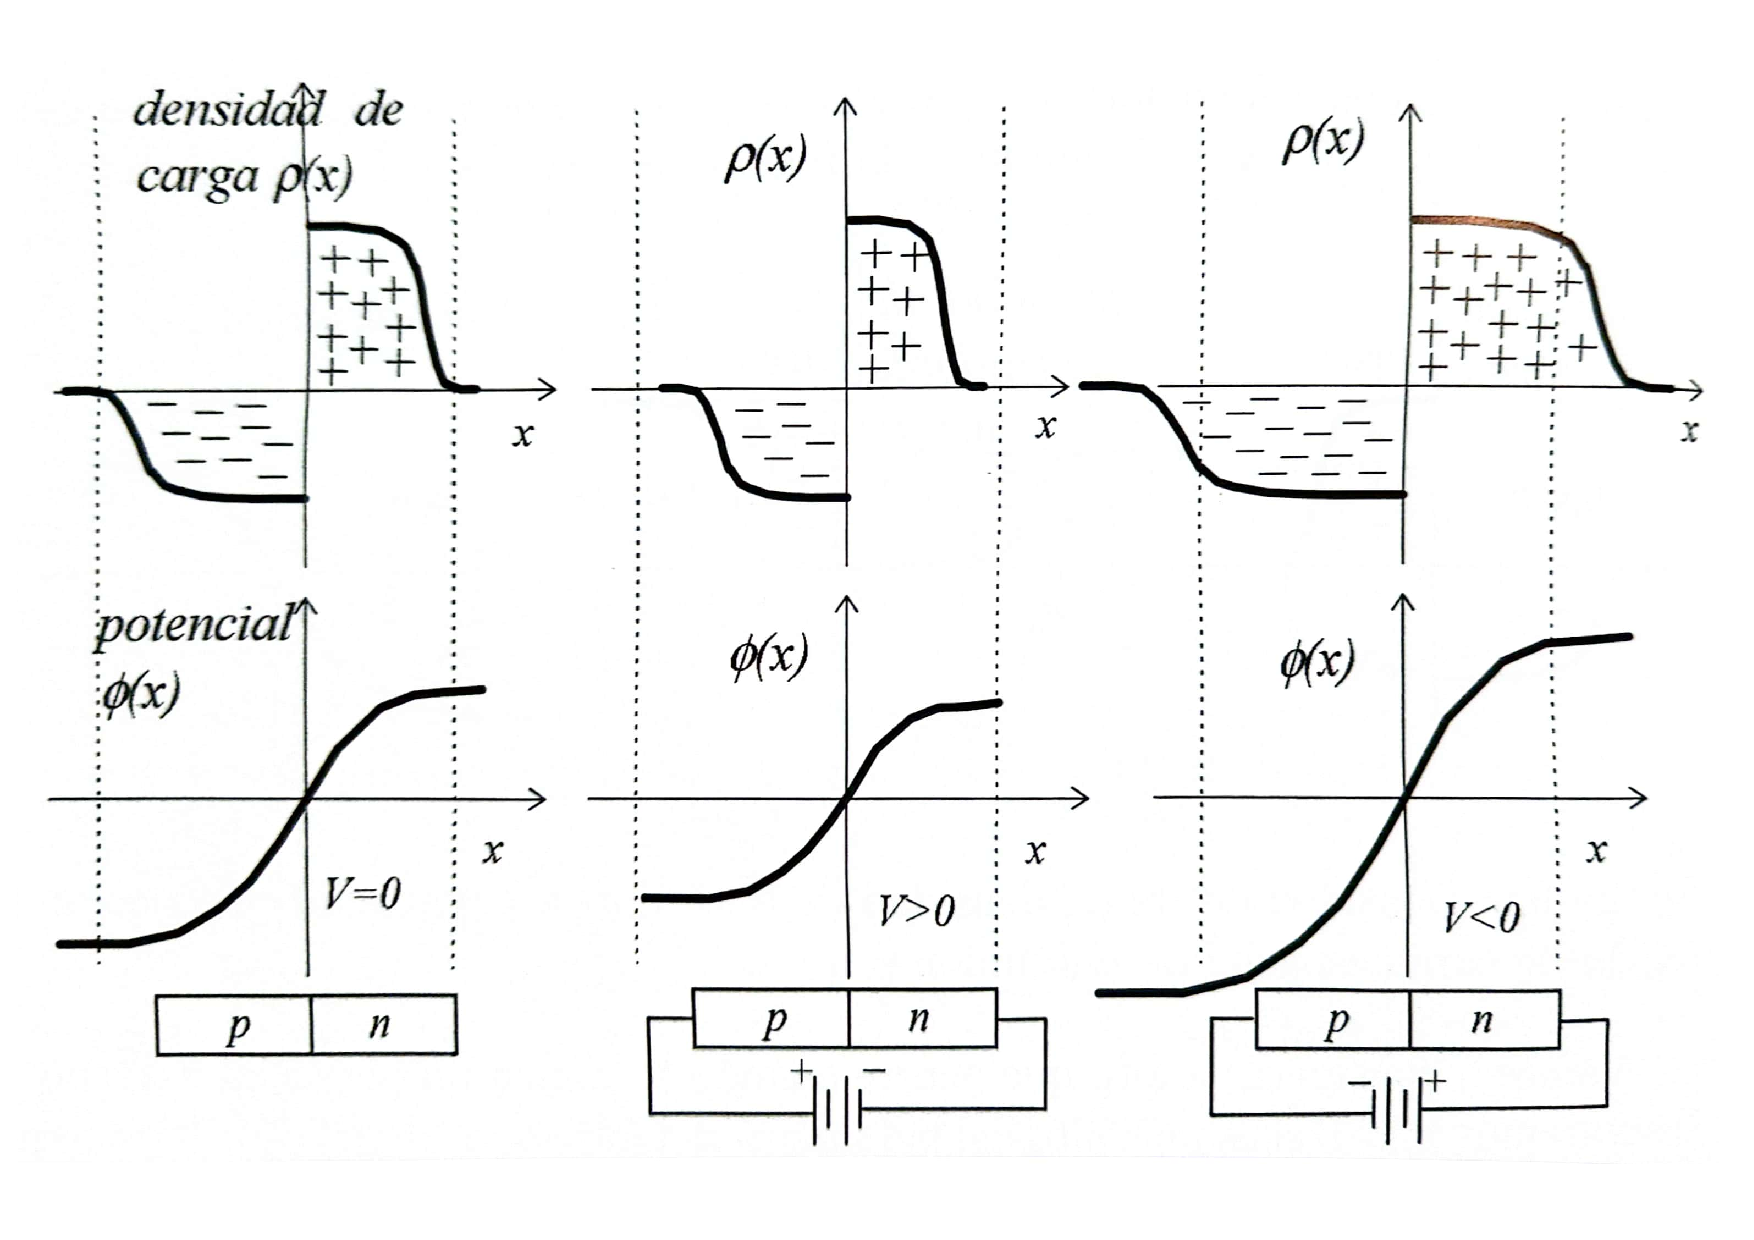
\includegraphics[scale=0.5]{Cuerpo/Ch_09/Fotos libro 7.pdf}
	\caption{}
	\label{Fig:09-07}
\end{figure}
\begin{figure}[h!] \centering
	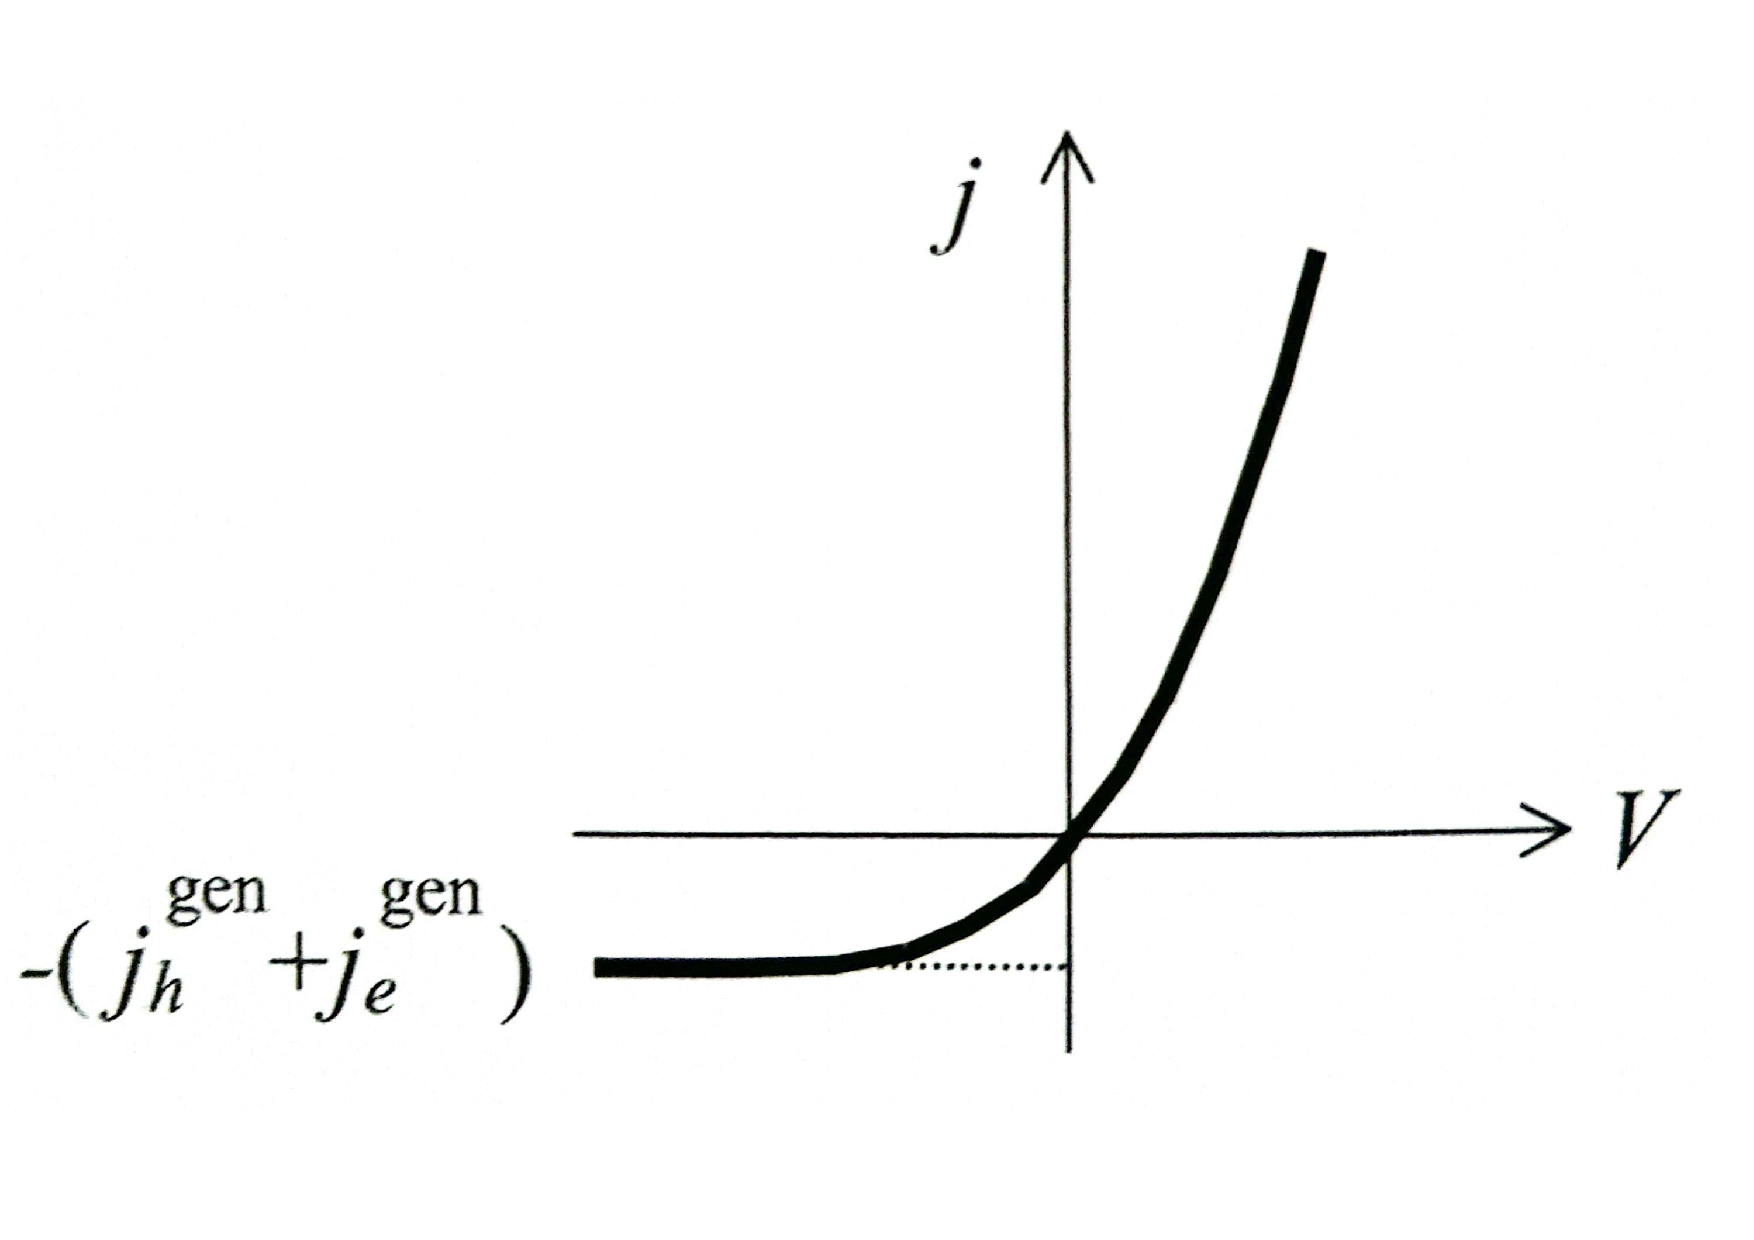
\includegraphics[scale=0.5]{Cuerpo/Ch_09/Fotos libro 8.pdf}
	\caption{}
	\label{Fig:09-08}
\end{figure}